\documentclass{standalone}

\begin{document}

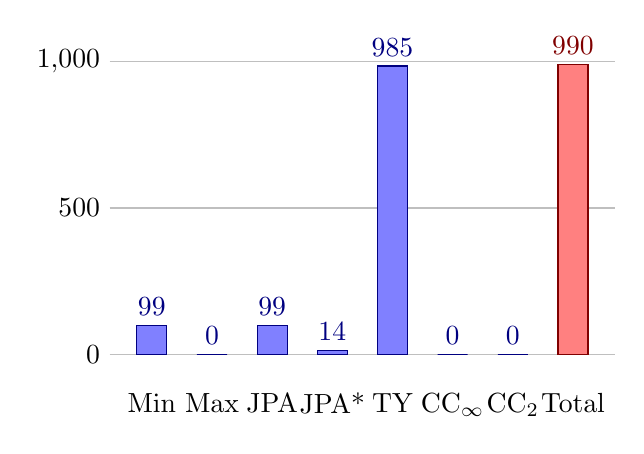
\begin{tikzpicture}
\begin{axis}[
    width=8cm,
    height=6cm,
    % Remove the frame
    axis line style={draw=none},
    % Remove the ticks
    tick style={draw=none},
    % Set the correct labels for the x axis
    xtick={1,2,3,4,5,6,7,8},
    xticklabels={Min,Max,JPA,JPA*,TY,$\mathrm{CC}_{\infty}$,$\mathrm{CC}_{2}$,Total},
    % Add major gridlines
    ymajorgrids=true,
    % Add labels on the bars
    nodes near coords,
    nodes near coords align={vertical},
    % Allow multiple plots in one
    every axis plot/.append style={
      ybar,
      bar width=.5,
      bar shift=0pt,
      fill
    }
]

  \addplot[blue!50!black,fill=blue!50] coordinates {(1,99) (2,0) (3,99) (4,14) (5,985) (6,0) (7,0)};
  \addplot[red!50!black,fill=red!50] coordinates {(8,990)};

\end{axis}
\end{tikzpicture}

\begin{tikzpicture}
\begin{axis}[
    width=8cm,
    height=6cm,
    mark size=1.5pt,
    axis lines=left,
]

  \addplot+[only marks, mark=x, black!50] table [x={Polynomial}, y={Period Length}, col sep=tab] {tables/period-length-ty.tsv};
  \addplot+[only marks, mark=star, red] table [x={Polynomial}, y={Period Length}, col sep=tab] {tables/period-length-mjpa.tsv};
  \addplot+[only marks, mark=o, blue] table [x={Polynomial}, y={Period Length}, col sep=tab] {tables/period-length-jpa.tsv};
  \addplot+[only marks, mark=+, blue] table [x={Polynomial}, y={Period Length}, col sep=tab] {tables/period-length-min.tsv};

  \legend{JPA,JPA*,TY,Min}

\end{axis}
\end{tikzpicture}

\end{document}

